\documentclass[aspectratio=169,xcolor={dvipsnames}]{beamer}

% Use UNIL theme
\usetheme{UNIL}

% Required packages
\usepackage{tikz}
\usepackage{listings}
\usepackage{array}
\usepackage{booktabs}
\usepackage{multirow}
\usepackage{amsmath}
\usepackage{amssymb}
\usepackage{subcaption}
\usepackage{pgfplots}

% TikZ libraries for diagrams
\usetikzlibrary{shapes,arrows,positioning,calc,fit,backgrounds,decorations.pathreplacing}

% PGFPlots version
\pgfplotsset{compat=1.17}

% Code listing style
\lstset{
    basicstyle=\ttfamily\small,
    keywordstyle=\color{blue},
    commentstyle=\color{gray},
    stringstyle=\color{red},
    showstringspaces=false,
    breaklines=true,
    frame=single,
    numbers=left,
    numberstyle=\tiny\color{gray},
    xleftmargin=2em,
    framexleftmargin=1.5em
}

% Define custom colors
\definecolor{codegreen}{rgb}{0,0.6,0}
\definecolor{codegray}{rgb}{0.5,0.5,0.5}
\definecolor{codepurple}{rgb}{0.58,0,0.82}
\definecolor{backcolour}{rgb}{0.95,0.95,0.92}

% Title information
\title{Foundations of High-Performance Computing (HPC)}
\subtitle{An Introduction to Parallel Computing and Cluster Computing}
\author{HPC Course}
\date{\today}

\begin{document}

% Title slide
\begin{frame}[plain]
    \titlepage
\end{frame}

% Table of contents
\begin{frame}{Course Overview}
    \tableofcontents
\end{frame}

%%%%%%%%%%%%%%%%%%%%%%%%%%%%%%%%%%%%%%%%%%%%%%%%%%%%%%%%%%%%%%%%%%%%%%%%%%
\section{Demystifying HPC Hardware}
%%%%%%%%%%%%%%%%%%%%%%%%%%%%%%%%%%%%%%%%%%%%%%%%%%%%%%%%%%%%%%%%%%%%%%%%%%

\begin{frame}{What is High-Performance Computing?}
    \begin{itemize}
        \item \textbf{High-Performance Computing (HPC)}: Using supercomputers and parallel processing techniques to solve complex computational problems
        \item \textbf{Goals:}
        \begin{itemize}
            \item Solve problems faster (reduced time to solution)
            \item Solve larger problems (increased problem size)
            \item Solve more problems simultaneously (increased throughput)
        \end{itemize}
        \item \textbf{Applications:}
        \begin{itemize}
            \item Weather forecasting and climate modeling
            \item Molecular dynamics and drug discovery
            \item Computational fluid dynamics
            \item Machine learning and AI
            \item Genomics and bioinformatics
        \end{itemize}
    \end{itemize}
\end{frame}

\begin{frame}{What is Parallel Computing?}
    \begin{itemize}
        \item \textbf{Parallel Computing}: Performing multiple operations at the same time
        \item A broad concept encompassing various forms of simultaneous computation
        \item \textbf{Core Idea:}
        \begin{itemize}
            \item Break down a task into smaller tasks
            \item Execute these smaller tasks simultaneously
            \item Combine results to get the final solution
        \end{itemize}
    \end{itemize}
\end{frame}

\begin{frame}{Parallelism vs Concurrency}
    \begin{columns}[T]
        \begin{column}{0.5\textwidth}
            \textbf{Concurrency:} Tasks that \emph{appear} to happen simultaneously but don't actually overlap in execution
            \vskip1em
            \textbf{Example: Learning to bike and talking on phone}
            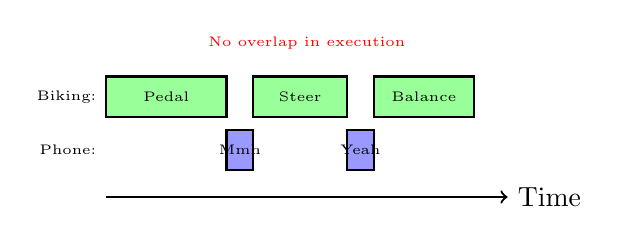
\begin{tikzpicture}[scale=0.85]
                % Time axis
                \draw[->, thick] (0,0) -- (6,0) node[right] {Time};
                
                % Biking task (learning - needs full attention)
                \node[left] at (0, 1.5) {\tiny Biking:};
                \draw[thick, fill=green!40] (0,1.2) rectangle (1.8,1.8);
                \node at (0.9, 1.5) {\tiny Pedal};
                \draw[thick, fill=green!40] (2.2,1.2) rectangle (3.6,1.8);
                \node at (2.9, 1.5) {\tiny Steer};
                \draw[thick, fill=green!40] (4.0,1.2) rectangle (5.5,1.8);
                \node at (4.75, 1.5) {\tiny Balance};
                
                % Phone task (brief responses)
                \node[left] at (0, 0.7) {\tiny Phone:};
                \draw[thick, fill=blue!40] (1.8,0.4) rectangle (2.2,1.0);
                \node at (2.0, 0.7) {\tiny Mmh};
                \draw[thick, fill=blue!40] (3.6,0.4) rectangle (4.0,1.0);
                \node at (3.8, 0.7) {\tiny Yeah};
                
                % No overlap indicator
                \node[red] at (3, 2.3) {\tiny No overlap in execution};
            \end{tikzpicture}
            \vskip0.5em
            Tasks alternate - only one executes at a time
        \end{column}
        \begin{column}{0.5\textwidth}
            \textbf{Parallelism:} Tasks that \emph{actually} execute at the same time
            \vskip1em
            \textbf{Example: Biking and talking on phone}
            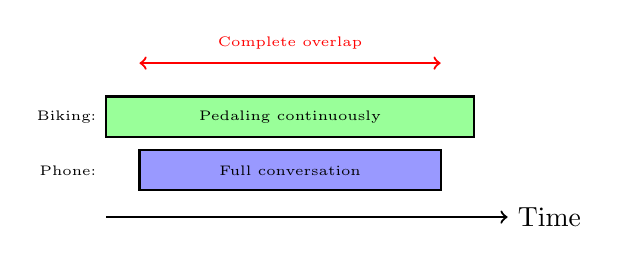
\begin{tikzpicture}[scale=0.85]
                % Time axis
                \draw[->, thick] (0,0) -- (6,0) node[right] {Time};
                
                % Biking task (continuous - experienced rider)
                \node[left] at (0, 1.5) {\tiny Biking:};
                \draw[thick, fill=green!40] (0,1.2) rectangle (5.5,1.8);
                \node at (2.75, 1.5) {\tiny Pedaling continuously};
                
                % Phone task (full conversation - overlapping)
                \node[left] at (0, 0.7) {\tiny Phone:};
                \draw[thick, fill=blue!40] (0.5,0.4) rectangle (5.0,1.0);
                \node at (2.75, 0.7) {\tiny Full conversation};
                
                % Overlap indicator
                \draw[red, thick, <->] (0.5, 2.3) -- (5.0, 2.3);
                \node[red] at (2.75, 2.6) {\tiny Complete overlap};
            \end{tikzpicture}
            \vskip0.5em
            Tasks execute simultaneously - true parallelism
        \end{column}
    \end{columns}
    \vskip1em
    \textbf{Key Distinction:} Concurrency is about \emph{dealing with} multiple things; parallelism is about \emph{doing} multiple things at once
\end{frame}

\begin{frame}{CPU Architecture Basics}
    \begin{columns}[T]
        \begin{column}{0.5\textwidth}
            \textbf{Key Components:}
            \begin{itemize}
                \item \textbf{CPU (Central Processing Unit)}: The main processor chip
                \item \textbf{Core}: An independent processing unit within a CPU
                \item \textbf{Socket}: Physical connector for a CPU on the motherboard
                \item \textbf{Thread}: Virtual core via hyperthreading/SMT
            \end{itemize}
        \end{column}
        \begin{column}{0.5\textwidth}
            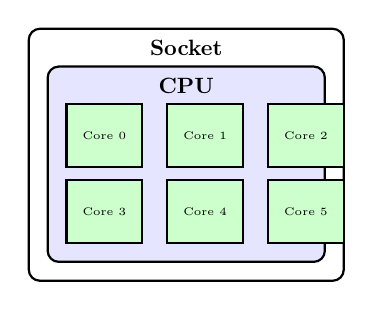
\begin{tikzpicture}[scale=0.8, every node/.style={scale=0.8}]
                % Socket
                \draw[thick, rounded corners] (0,0) rectangle (5,4);
                \node at (2.5, 3.7) {\textbf{Socket}};
                
                % CPU
                \draw[thick, rounded corners, fill=blue!10] (0.3,0.3) rectangle (4.7,3.4);
                \node at (2.5, 3.1) {\textbf{CPU}};
                
                % Cores
                \draw[thick, fill=green!20] (0.6,1.8) rectangle (1.8,2.8);
                \node at (1.2, 2.3) {\tiny Core 0};
                
                \draw[thick, fill=green!20] (2.2,1.8) rectangle (3.4,2.8);
                \node at (2.8, 2.3) {\tiny Core 1};
                
                \draw[thick, fill=green!20] (3.8,1.8) rectangle (5.0,2.8);
                \node at (4.4, 2.3) {\tiny Core 2};
                
                \draw[thick, fill=green!20] (0.6,0.6) rectangle (1.8,1.6);
                \node at (1.2, 1.1) {\tiny Core 3};
                
                \draw[thick, fill=green!20] (2.2,0.6) rectangle (3.4,1.6);
                \node at (2.8, 1.1) {\tiny Core 4};
                
                \draw[thick, fill=green!20] (3.8,0.6) rectangle (5.0,1.6);
                \node at (4.4, 1.1) {\tiny Core 5};
            \end{tikzpicture}
        \end{column}
    \end{columns}
    \vskip1em
    \textbf{Example:} A dual-socket server with 2 CPUs × 64 cores/CPU = 128 cores total
\end{frame}

\begin{frame}{Memory Hierarchy}
    \begin{columns}[T]
        \begin{column}{0.5\textwidth}
            \textbf{Levels of Memory:}
            \begin{enumerate}
                \item \textbf{Registers}: Fastest, smallest (bytes)
                \item \textbf{L1 Cache}: Very fast, per-core (KB)
                \item \textbf{L2 Cache}: Fast, per-core (KB)
                \item \textbf{L3 Cache}: Shared, per-CPU (MB)
                \item \textbf{Main Memory (RAM)}: Large (GB)
                \item \textbf{Storage (Disk)}: Largest, slowest (TB)
            \end{enumerate}
            \vskip0.5em
            \textbf{Key Principle:} Faster memory is smaller and more expensive
        \end{column}
        \begin{column}{0.5\textwidth}
            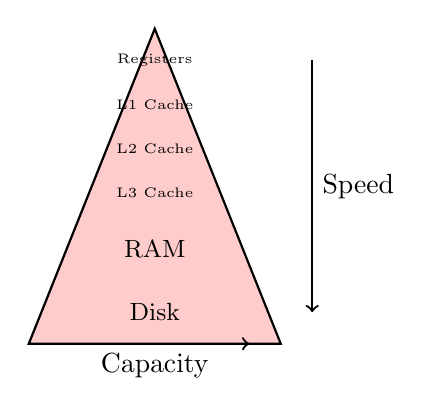
\begin{tikzpicture}[scale=0.8]
                % Triangle representing hierarchy
                \draw[thick, fill=red!20] (0,0) -- (4,0) -- (2,5) -- cycle;
                
                % Labels
                \node at (2, 4.5) {\tiny Registers};
                \node at (2, 3.8) {\tiny L1 Cache};
                \node at (2, 3.1) {\tiny L2 Cache};
                \node at (2, 2.4) {\tiny L3 Cache};
                \node at (2, 1.5) {\small RAM};
                \node at (2, 0.5) {\small Disk};
                
                % Arrows for speed and size
                \draw[->, thick] (4.5, 4.5) -- (4.5, 0.5) node[midway, right] {Speed};
                \draw[->, thick] (0.5, 0) -- (3.5, 0) node[midway, below] {Capacity};
            \end{tikzpicture}
        \end{column}
    \end{columns}
\end{frame}

\begin{frame}{Shared vs Distributed Memory}
    \begin{columns}[T]
        \begin{column}{0.5\textwidth}
            \textbf{Shared Memory:}
            \begin{itemize}
                \item All cores access same RAM
                \item Fast communication
                \item Limited scalability
                \item Example: Multi-core CPU
            \end{itemize}
            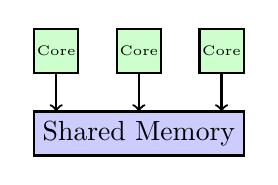
\begin{tikzpicture}[scale=0.7]
                % Cores
                \foreach \x in {0,1.5,3} {
                    \draw[thick, fill=green!20] (\x,2) rectangle (\x+0.8,2.8);
                    \node at (\x+0.4, 2.4) {\tiny Core};
                }
                % Shared memory
                \draw[thick, fill=blue!20] (0,0.5) rectangle (3.8,1.3);
                \node at (1.9, 0.9) {Shared Memory};
                % Arrows
                \foreach \x in {0.4,1.9,3.4} {
                    \draw[->, thick] (\x, 2) -- (\x, 1.3);
                }
            \end{tikzpicture}
        \end{column}
        \begin{column}{0.5\textwidth}
            \textbf{Distributed Memory:}
            \begin{itemize}
                \item Each node has own RAM
                \item Explicit data transfer (MPI)
                \item Highly scalable
                \item Example: HPC cluster
            \end{itemize}
            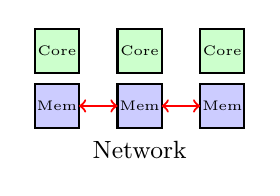
\begin{tikzpicture}[scale=0.7]
                % Node 1
                \draw[thick, fill=green!20] (0,2.5) rectangle (0.8,3.3);
                \node at (0.4, 2.9) {\tiny Core};
                \draw[thick, fill=blue!20] (0,1.5) rectangle (0.8,2.3);
                \node at (0.4, 1.9) {\tiny Mem};
                
                % Node 2
                \draw[thick, fill=green!20] (1.5,2.5) rectangle (2.3,3.3);
                \node at (1.9, 2.9) {\tiny Core};
                \draw[thick, fill=blue!20] (1.5,1.5) rectangle (2.3,2.3);
                \node at (1.9, 1.9) {\tiny Mem};
                
                % Node 3
                \draw[thick, fill=green!20] (3,2.5) rectangle (3.8,3.3);
                \node at (3.4, 2.9) {\tiny Core};
                \draw[thick, fill=blue!20] (3,1.5) rectangle (3.8,2.3);
                \node at (3.4, 1.9) {\tiny Mem};
                
                % Network
                \draw[thick, <->, red] (0.8, 1.9) -- (1.5, 1.9);
                \draw[thick, <->, red] (2.3, 1.9) -- (3, 1.9);
                \node at (1.9, 1.1) {\small Network};
            \end{tikzpicture}
        \end{column}
    \end{columns}
\end{frame}

\begin{frame}{Compute Nodes in an HPC Cluster}
    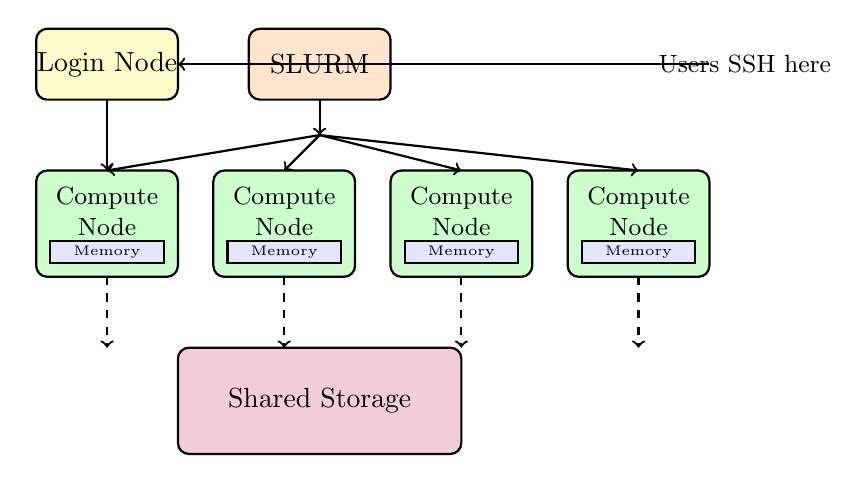
\begin{tikzpicture}[scale=0.9]
        % Login node
        \draw[thick, fill=yellow!20, rounded corners] (0,5) rectangle (2,6);
        \node at (1, 5.5) {Login Node};
        
        % Scheduler
        \draw[thick, fill=orange!20, rounded corners] (3,5) rectangle (5,6);
        \node at (4, 5.5) {SLURM};
        
        % Compute nodes
        \foreach \x in {0,2.5,5,7.5} {
            \draw[thick, fill=green!20, rounded corners] (\x,2.5) rectangle (\x+2,4);
            \node at (\x+1, 3.6) {\small Compute};
            \node at (\x+1, 3.2) {\small Node};
            \draw[thick, fill=blue!10] (\x+0.2,2.7) rectangle (\x+1.8,3);
            \node at (\x+1, 2.85) {\tiny Memory};
        }
        
        % Storage
        \draw[thick, fill=purple!20, rounded corners] (2,0) rectangle (6,1.5);
        \node at (4, 0.75) {Shared Storage};
        
        % Arrows
        \draw[->, thick] (1, 5) -- (1, 4);
        \draw[->, thick] (4, 5) -- (4, 4.5);
        \draw[->, thick] (4, 4.5) -- (1, 4);
        \draw[->, thick] (4, 4.5) -- (3.5, 4);
        \draw[->, thick] (4, 4.5) -- (6, 4);
        \draw[->, thick] (4, 4.5) -- (8.5, 4);
        
        % Storage connections
        \foreach \x in {1,3.5,6,8.5} {
            \draw[->, thick, dashed] (\x, 2.5) -- (\x, 1.5);
        }
        
        \node at (10, 5.5) {\small Users SSH here};
        \draw[->, thick] (9.5, 5.5) -- (2, 5.5);
    \end{tikzpicture}
    
    \vskip0.5em
    \textbf{Workflow:} Users connect to login node → Submit jobs to SLURM → Jobs run on compute nodes
\end{frame}

\begin{frame}{SLURM Terminology: CPUs vs Tasks}
    \begin{columns}[T]
        \begin{column}{0.5\textwidth}
            \textbf{Key Terms:}
            \begin{itemize}
                \item \textbf{Node}: A single computer in the cluster
                \item \textbf{CPU}: In SLURM, often means a "core"
                \item \textbf{Task}: A process (instance of a program)
                \item \textbf{CPUs per task}: Cores available to each task
            \end{itemize}
            \vskip1em
            \textbf{Important:} 
            \begin{itemize}
                \item SLURM's "cpu" ≠ physical CPU
                \item Usually means a core or hardware thread
                \item Check your cluster's definition!
            \end{itemize}
        \end{column}
        \begin{column}{0.5\textwidth}
            \textbf{Example Configurations:}
            \vskip0.5em
            \begin{tabular}{lcc}
                \toprule
                \textbf{Config} & \textbf{Tasks} & \textbf{CPUs/Task} \\
                \midrule
                Serial & 1 & 1 \\
                Multi-threaded & 1 & 16 \\
                MPI & 32 & 1 \\
                Hybrid & 4 & 8 \\
                \bottomrule
            \end{tabular}
            \vskip1em
            \textbf{Resource Calculation:}
            \begin{itemize}
                \item Total CPUs = Tasks × CPUs per task
                \item Example: 4 tasks × 8 CPUs = 32 cores
            \end{itemize}
        \end{column}
    \end{columns}
\end{frame}

\begin{frame}{Understanding Resource Allocation}
    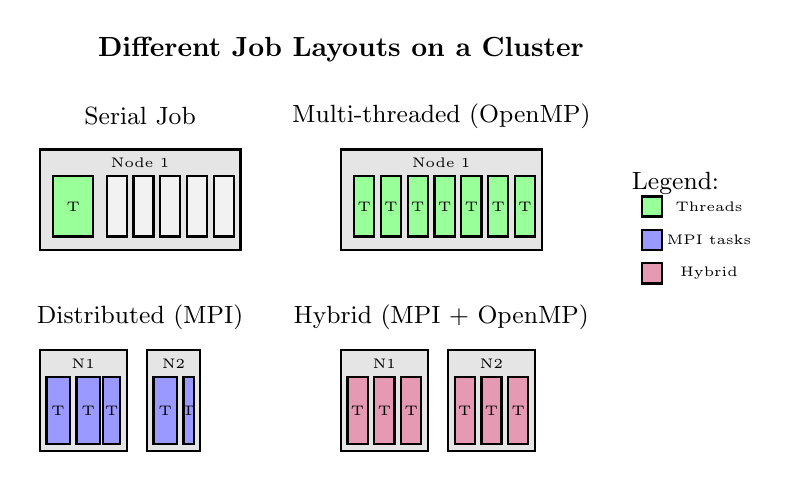
\begin{tikzpicture}[scale=0.85]
        % Title
        \node at (5, 6.5) {\textbf{Different Job Layouts on a Cluster}};
        
        % Single Node - Serial Job
        \node at (2, 5.5) {\small Serial Job};
        \draw[thick, fill=gray!20] (0.5,3.5) rectangle (3.5,5);
        \node at (2, 4.8) {\tiny Node 1};
        \draw[thick, fill=green!40] (0.7,3.7) rectangle (1.3,4.6);
        \node at (1, 4.15) {\tiny T};
        \foreach \x in {1.5,1.9,2.3,2.7,3.1} {
            \draw[thick, fill=gray!10] (\x,3.7) rectangle (\x+0.3,4.6);
        }
        
        % Multi-threaded Job
        \node at (6.5, 5.5) {\small Multi-threaded (OpenMP)};
        \draw[thick, fill=gray!20] (5,3.5) rectangle (8,5);
        \node at (6.5, 4.8) {\tiny Node 1};
        \foreach \x in {5.2,5.6,6.0,6.4,6.8,7.2,7.6} {
            \draw[thick, fill=green!40] (\x,3.7) rectangle (\x+0.3,4.6);
            \node at (\x+0.15, 4.15) {\tiny T};
        }
        
        % Distributed MPI Job
        \node at (2, 2.5) {\small Distributed (MPI)};
        \draw[thick, fill=gray!20] (0.5,0.5) rectangle (1.8,2);
        \node at (1.15, 1.8) {\tiny N1};
        \draw[thick, fill=blue!40] (0.6,0.6) rectangle (0.95,1.6);
        \node at (0.775, 1.1) {\tiny T};
        \draw[thick, fill=blue!40] (1.05,0.6) rectangle (1.4,1.6);
        \node at (1.225, 1.1) {\tiny T};
        \draw[thick, fill=blue!40] (1.45,0.6) rectangle (1.7,1.6);
        \node at (1.575, 1.1) {\tiny T};
        
        \draw[thick, fill=gray!20] (2.1,0.5) rectangle (2.9,2);
        \node at (2.5, 1.8) {\tiny N2};
        \draw[thick, fill=blue!40] (2.2,0.6) rectangle (2.55,1.6);
        \node at (2.375, 1.1) {\tiny T};
        \draw[thick, fill=blue!40] (2.65,0.6) rectangle (2.8,1.6);
        \node at (2.725, 1.1) {\tiny T};
        
        % Hybrid Job
        \node at (6.5, 2.5) {\small Hybrid (MPI + OpenMP)};
        \draw[thick, fill=gray!20] (5,0.5) rectangle (6.3,2);
        \node at (5.65, 1.8) {\tiny N1};
        \foreach \x in {5.1,5.5,5.9} {
            \draw[thick, fill=purple!40] (\x,0.6) rectangle (\x+0.3,1.6);
            \node at (\x+0.15, 1.1) {\tiny T};
        }
        
        \draw[thick, fill=gray!20] (6.6,0.5) rectangle (7.9,2);
        \node at (7.25, 1.8) {\tiny N2};
        \foreach \x in {6.7,7.1,7.5} {
            \draw[thick, fill=purple!40] (\x,0.6) rectangle (\x+0.3,1.6);
            \node at (\x+0.15, 1.1) {\tiny T};
        }
        
        % Legend
        \node at (10, 4.5) {\small Legend:};
        \draw[thick, fill=green!40] (9.5,4) rectangle (9.8,4.3);
        \node at (10.5, 4.15) {\tiny Threads};
        \draw[thick, fill=blue!40] (9.5,3.5) rectangle (9.8,3.8);
        \node at (10.5, 3.65) {\tiny MPI tasks};
        \draw[thick, fill=purple!40] (9.5,3) rectangle (9.8,3.3);
        \node at (10.5, 3.15) {\tiny Hybrid};
    \end{tikzpicture}
\end{frame}

%%%%%%%%%%%%%%%%%%%%%%%%%%%%%%%%%%%%%%%%%%%%%%%%%%%%%%%%%%%%%%%%%%%%%%%%%%
\section{Understanding Parallelism}
%%%%%%%%%%%%%%%%%%%%%%%%%%%%%%%%%%%%%%%%%%%%%%%%%%%%%%%%%%%%%%%%%%%%%%%%%%

\begin{frame}{Why Parallel Computing?}
    \begin{columns}[T]
        \begin{column}{0.5\textwidth}
            \textbf{Serial Computing Limitations:}
            \begin{itemize}
                \item CPU clock speeds plateaued (~2005)
                \item Physical limits (power, heat)
                \item Need for faster solutions
            \end{itemize}
            \vskip1em
            \textbf{Solution: Parallelism}
            \begin{itemize}
                \item Use multiple cores simultaneously
                \item Divide work among processors
                \item Reduce time to solution
            \end{itemize}
        \end{column}
        \begin{column}{0.5\textwidth}
            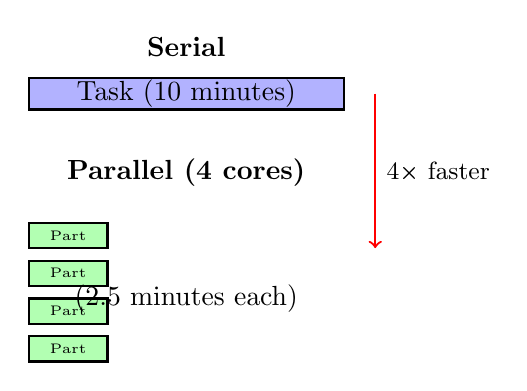
\begin{tikzpicture}[scale=0.8]
                % Serial execution
                \node at (2.5, 5) {\textbf{Serial}};
                \draw[thick, fill=blue!30] (0,4) rectangle (5,4.5);
                \node at (2.5, 4.25) {Task (10 minutes)};
                
                % Parallel execution
                \node at (2.5, 3) {\textbf{Parallel (4 cores)}};
                \foreach \y in {0,0.6,1.2,1.8} {
                    \draw[thick, fill=green!30] (0,\y) rectangle (1.25,\y+0.4);
                    \node at (0.625, \y+0.2) {\tiny Part};
                }
                \node at (2.5, 1) {(2.5 minutes each)};
                
                % Speedup arrow
                \draw[->, thick, red] (5.5, 4.25) -- (5.5, 1.8);
                \node at (6.5, 3) {\small 4× faster};
            \end{tikzpicture}
            \vskip0.5em
            \textbf{Note:} Ideal speedup is rarely achieved due to overhead and serial portions
        \end{column}
    \end{columns}
\end{frame}

\begin{frame}{Levels of Parallelism}
    \begin{enumerate}
        \item \textbf{Instruction-Level Parallelism (ILP)}
        \begin{itemize}
            \item Pipelining and out-of-order execution
            \item Automatic (hardware-level)
            \item Not programmable by users
        \end{itemize}
        \vskip0.5em
        
        \item \textbf{Vectorization (SIMD)}
        \begin{itemize}
            \item Single Instruction, Multiple Data
            \item Process multiple data elements simultaneously
            \item Compiler can auto-vectorize or use intrinsics
        \end{itemize}
        \vskip0.5em
        
        \item \textbf{Thread-Level Parallelism (Shared Memory)}
        \begin{itemize}
            \item Multiple threads on same node
            \item OpenMP, pthreads, threading libraries
            \item Access shared memory space
        \end{itemize}
        \vskip0.5em
        
        \item \textbf{Process-Level Parallelism (Distributed Memory)}
        \begin{itemize}
            \item Multiple processes across nodes
            \item MPI (Message Passing Interface)
            \item Explicit communication between processes
        \end{itemize}
    \end{enumerate}
\end{frame}


\begin{frame}{Vectorization (SIMD)}
    \begin{columns}[T]
        \begin{column}{0.5\textwidth}
            \textbf{Concept:} Apply same operation to multiple data elements simultaneously
            \vskip1em
            \textbf{Example: Vector Addition}
            \begin{align*}
                C[0:3] = A[0:3] + B[0:3]
            \end{align*}
            \vskip0.5em
            \textbf{Without SIMD:}
            \begin{itemize}
                \item 4 separate additions
                \item 4 clock cycles
            \end{itemize}
            \vskip0.5em
            \textbf{With SIMD:}
            \begin{itemize}
                \item 1 vector addition
                \item 1 clock cycle
                \item 4× speedup!
            \end{itemize}
        \end{column}
        \begin{column}{0.5\textwidth}
            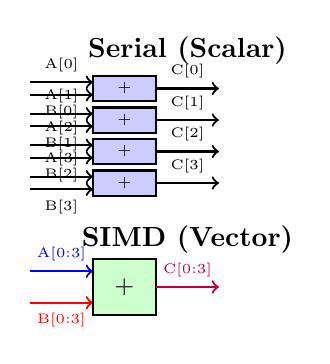
\begin{tikzpicture}[scale=0.8]
                % Serial
                \node at (2.5, 5.5) {\textbf{Serial (Scalar)}};
                \foreach \y/\n in {5/0,4.5/1,4/2,3.5/3} {
                    \draw[->, thick] (0,\y) -- (1,\y) node[midway, above] {\tiny A[\n]};
                    \draw[->, thick] (0,\y-0.2) -- (1,\y-0.2) node[midway, below] {\tiny B[\n]};
                    \draw[thick, fill=blue!20] (1,\y-0.3) rectangle (2,\y+0.1);
                    \node at (1.5, \y-0.1) {\tiny +};
                    \draw[->, thick] (2,\y-0.1) -- (3,\y-0.1) node[midway, above] {\tiny C[\n]};
                }
                
                % SIMD
                \node at (2.5, 2.5) {\textbf{SIMD (Vector)}};
                \draw[->, thick, blue] (0,2) -- (1,2) node[midway, above] {\tiny A[0:3]};
                \draw[->, thick, red] (0,1.5) -- (1,1.5) node[midway, below] {\tiny B[0:3]};
                \draw[thick, fill=green!20] (1,1.3) rectangle (2,2.2);
                \node at (1.5, 1.75) {\small +};
                \draw[->, thick, purple] (2,1.75) -- (3,1.75) node[midway, above] {\tiny C[0:3]};
            \end{tikzpicture}
            \vskip0.5em
            \textbf{Modern CPUs:}
            \begin{itemize}
                \item AVX-512: 512-bit vectors
                \item Process 16 floats at once
            \end{itemize}
        \end{column}
    \end{columns}
\end{frame}

\begin{frame}[fragile]{Multi-Threading (Shared Memory)}
    \begin{columns}[T]
        \begin{column}{0.5\textwidth}
            \textbf{Thread-Level Parallelism:}
            \begin{itemize}
                \item Multiple threads in same process
                \item Share memory address space
                \item Lightweight context switching
                \item Common APIs: OpenMP, pthreads, C++ threads
            \end{itemize}
            \vskip1em
            \textbf{OpenMP Example:}
            \begin{lstlisting}[language=C, basicstyle=\tiny\ttfamily]
#pragma omp parallel for
for (int i = 0; i < N; i++) {
    c[i] = a[i] + b[i];
}
            \end{lstlisting}
        \end{column}
        \begin{column}{0.5\textwidth}
            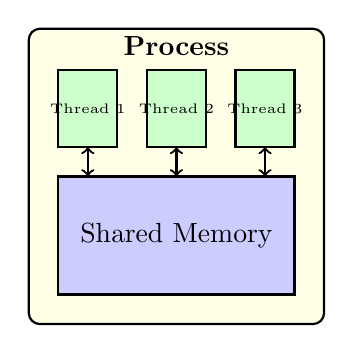
\begin{tikzpicture}[scale=0.75]
                % Process
                \draw[thick, rounded corners, fill=yellow!10] (0,0) rectangle (5,5);
                \node at (2.5, 4.7) {\textbf{Process}};
                
                % Threads
                \draw[thick, fill=green!20] (0.5,3) rectangle (1.5,4.3);
                \node at (1, 3.65) {\tiny Thread 1};
                
                \draw[thick, fill=green!20] (2,3) rectangle (3,4.3);
                \node at (2.5, 3.65) {\tiny Thread 2};
                
                \draw[thick, fill=green!20] (3.5,3) rectangle (4.5,4.3);
                \node at (4, 3.65) {\tiny Thread 3};
                
                % Shared memory
                \draw[thick, fill=blue!20] (0.5,0.5) rectangle (4.5,2.5);
                \node at (2.5, 1.5) {Shared Memory};
                
                % Arrows
                \draw[<->, thick] (1, 3) -- (1, 2.5);
                \draw[<->, thick] (2.5, 3) -- (2.5, 2.5);
                \draw[<->, thick] (4, 3) -- (4, 2.5);
            \end{tikzpicture}
            \vskip0.5em
            \textbf{Benefits:} Fast communication, easy data sharing
        \end{column}
    \end{columns}
\end{frame}

\begin{frame}{Message Passing (Distributed Memory)}
    \begin{columns}[T]
        \begin{column}{0.5\textwidth}
            \textbf{Message Passing Interface (MPI):}
            \begin{itemize}
                \item Multiple processes with separate memory
                \item Explicit communication via messages
                \item Scales across many nodes
                \item Standard library with many implementations
            \end{itemize}
            \vskip1em
            \textbf{Key Operations:}
            \begin{itemize}
                \item \texttt{MPI\_Send}: Send data
                \item \texttt{MPI\_Recv}: Receive data
                \item \texttt{MPI\_Bcast}: Broadcast to all
                \item \texttt{MPI\_Reduce}: Collect and combine
            \end{itemize}
        \end{column}
        \begin{column}{0.5\textwidth}
            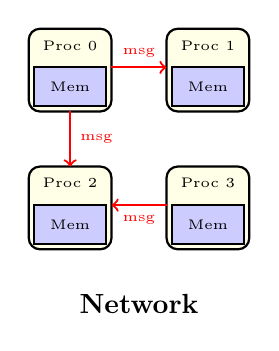
\begin{tikzpicture}[scale=0.7]
                % Process 0
                \draw[thick, rounded corners, fill=yellow!10] (0,4) rectangle (1.5,5.5);
                \node at (0.75, 5.2) {\tiny Proc 0};
                \draw[thick, fill=blue!20] (0.1,4.1) rectangle (1.4,4.8);
                \node at (0.75, 4.45) {\tiny Mem};
                
                % Process 1
                \draw[thick, rounded corners, fill=yellow!10] (2.5,4) rectangle (4,5.5);
                \node at (3.25, 5.2) {\tiny Proc 1};
                \draw[thick, fill=blue!20] (2.6,4.1) rectangle (3.9,4.8);
                \node at (3.25, 4.45) {\tiny Mem};
                
                % Process 2
                \draw[thick, rounded corners, fill=yellow!10] (0,1.5) rectangle (1.5,3);
                \node at (0.75, 2.7) {\tiny Proc 2};
                \draw[thick, fill=blue!20] (0.1,1.6) rectangle (1.4,2.3);
                \node at (0.75, 1.95) {\tiny Mem};
                
                % Process 3
                \draw[thick, rounded corners, fill=yellow!10] (2.5,1.5) rectangle (4,3);
                \node at (3.25, 2.7) {\tiny Proc 3};
                \draw[thick, fill=blue!20] (2.6,1.6) rectangle (3.9,2.3);
                \node at (3.25, 1.95) {\tiny Mem};
                
                % Communication arrows
                \draw[->, thick, red] (1.5, 4.8) -- (2.5, 4.8) node[midway, above] {\tiny msg};
                \draw[->, thick, red] (0.75, 4) -- (0.75, 3) node[midway, right] {\tiny msg};
                \draw[->, thick, red] (2.5, 2.3) -- (1.5, 2.3) node[midway, below] {\tiny msg};
                
                % Network
                \node at (2, 0.5) {\textbf{Network}};
            \end{tikzpicture}
            \vskip0.5em
            \textbf{Trade-off:} More complex but highly scalable
        \end{column}
    \end{columns}
\end{frame}

\begin{frame}{Hybrid Parallelization}
    \begin{columns}[T]
        \begin{column}{0.5\textwidth}
            \textbf{Combining MPI + OpenMP:}
            \begin{itemize}
                \item MPI for inter-node communication
                \item OpenMP for intra-node parallelism
                \item Best of both worlds
                \item Common in modern HPC applications
            \end{itemize}
            \vskip1em
            \textbf{Benefits:}
            \begin{itemize}
                \item Reduced message passing overhead
                \item Better memory utilization
                \item Improved scalability
                \item Flexible resource allocation
            \end{itemize}
        \end{column}
        \begin{column}{0.5\textwidth}
            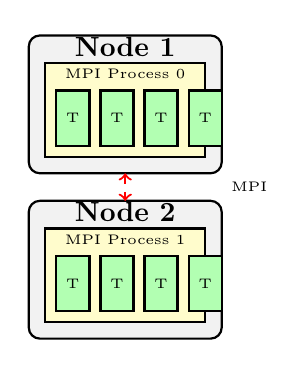
\begin{tikzpicture}[scale=0.7]
                % Node 1
                \draw[thick, rounded corners, fill=gray!10] (0,3) rectangle (3.5,5.5);
                \node at (1.75, 5.3) {\textbf{Node 1}};
                
                % MPI process 1
                \draw[thick, fill=yellow!20] (0.3,3.3) rectangle (3.2,5);
                \node at (1.75, 4.8) {\tiny MPI Process 0};
                
                % OpenMP threads
                \foreach \x in {0.5,1.3,2.1,2.9} {
                    \draw[thick, fill=green!30] (\x,3.5) rectangle (\x+0.6,4.5);
                    \node at (\x+0.3, 4) {\tiny T};
                }
                
                % Node 2
                \draw[thick, rounded corners, fill=gray!10] (0,0) rectangle (3.5,2.5);
                \node at (1.75, 2.3) {\textbf{Node 2}};
                
                % MPI process 2
                \draw[thick, fill=yellow!20] (0.3,0.3) rectangle (3.2,2);
                \node at (1.75, 1.8) {\tiny MPI Process 1};
                
                % OpenMP threads
                \foreach \x in {0.5,1.3,2.1,2.9} {
                    \draw[thick, fill=green!30] (\x,0.5) rectangle (\x+0.6,1.5);
                    \node at (\x+0.3, 1) {\tiny T};
                }
                
                % MPI communication
                \draw[<->, thick, red, dashed] (1.75, 3) -- (1.75, 2.5);
                \node at (4, 2.75) {\tiny MPI};
            \end{tikzpicture}
        \end{column}
    \end{columns}
    \vskip0.5em
    \textbf{Example:} 2 nodes × 4 threads = 8 total cores, but only 2 MPI processes
\end{frame}

\begin{frame}[fragile]{Amdahl's Law: The Speedup Limit}
    \begin{columns}[T]
        \begin{column}{0.5\textwidth}
            \textbf{Key Insight:}
            \begin{itemize}
                \item Speedup is limited by serial portion of code
                \item Not all code can be parallelized
                \item Adding more processors has diminishing returns
            \end{itemize}
            \vskip1em
            \textbf{Formula:}
            \[
            S(n) = \frac{1}{(1-p) + \frac{p}{n}}
            \]
            where:
            \begin{itemize}
                \item $S(n)$ = speedup with $n$ processors
                \item $p$ = parallel fraction of code
                \item $(1-p)$ = serial fraction
            \end{itemize}
        \end{column}
        \begin{column}{0.5\textwidth}
            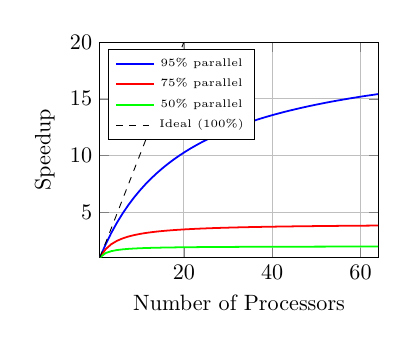
\begin{tikzpicture}[scale=0.8]
                \begin{axis}[
                    width=6cm,
                    height=5cm,
                    xlabel={Number of Processors},
                    ylabel={Speedup},
                    legend pos=north west,
                    grid=major,
                    xmin=1, xmax=64,
                    ymin=1, ymax=20,
                    legend style={font=\tiny}
                ]
                \addplot[blue, thick, domain=1:64, samples=50] {1/((1-0.95) + 0.95/x)};
                \addlegendentry{95\% parallel}
                
                \addplot[red, thick, domain=1:64, samples=50] {1/((1-0.75) + 0.75/x)};
                \addlegendentry{75\% parallel}
                
                \addplot[green, thick, domain=1:64, samples=50] {1/((1-0.50) + 0.50/x)};
                \addlegendentry{50\% parallel}
                
                \addplot[black, dashed, domain=1:64] {x};
                \addlegendentry{Ideal (100\%)}
                \end{axis}
            \end{tikzpicture}
            \vskip0.5em
            \textbf{Lesson:} Optimize serial portions first!
        \end{column}
    \end{columns}
\end{frame}

%%%%%%%%%%%%%%%%%%%%%%%%%%%%%%%%%%%%%%%%%%%%%%%%%%%%%%%%%%%%%%%%%%%%%%%%%%
\section{Cluster Workflow and SLURM Basics}
%%%%%%%%%%%%%%%%%%%%%%%%%%%%%%%%%%%%%%%%%%%%%%%%%%%%%%%%%%%%%%%%%%%%%%%%%%

\begin{frame}{What is SLURM?}
    \textbf{Simple Linux Utility for Resource Management}
    \vskip1em
    \begin{columns}[T]
        \begin{column}{0.5\textwidth}
            \textbf{Functions:}
            \begin{itemize}
                \item \textbf{Resource Manager}: Allocate compute resources
                \item \textbf{Job Scheduler}: Queue and prioritize jobs
                \item \textbf{Workload Manager}: Monitor job execution
            \end{itemize}
            \vskip1em
            \textbf{Why SLURM?}
            \begin{itemize}
                \item Fair sharing of resources
                \item Prevents conflicts
                \item Optimizes cluster utilization
                \item Provides accounting and reporting
            \end{itemize}
        \end{column}
        \begin{column}{0.5\textwidth}
            \textbf{Job Lifecycle:}
            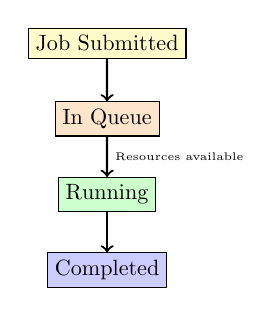
\begin{tikzpicture}[node distance=1.2cm, scale=0.7, every node/.style={scale=0.8}]
                \node[draw, rectangle, fill=yellow!20] (submit) {Job Submitted};
                \node[draw, rectangle, fill=orange!20, below of=submit] (queue) {In Queue};
                \node[draw, rectangle, fill=green!20, below of=queue] (run) {Running};
                \node[draw, rectangle, fill=blue!20, below of=run] (complete) {Completed};
                
                \draw[->, thick] (submit) -- (queue);
                \draw[->, thick] (queue) -- (run) node[midway, right] {\tiny Resources available};
                \draw[->, thick] (run) -- (complete);
            \end{tikzpicture}
        \end{column}
    \end{columns}
\end{frame}

\begin{frame}{Common SLURM Commands}
    \begin{tabular}{p{3.5cm}p{7cm}}
        \toprule
        \textbf{Command} & \textbf{Description} \\
        \midrule
        \texttt{sbatch script.sh} & Submit a batch job \\
        \texttt{squeue} & View job queue (all users) \\
        \texttt{squeue -u \$USER} & View your jobs \\
        \texttt{scancel <jobid>} & Cancel a job \\
        \texttt{sinfo} & View cluster node information \\
        \texttt{srun command} & Run command interactively \\
        \texttt{scontrol show job <jobid>} & View detailed job info \\
        \texttt{sacct} & View job accounting information \\
        \texttt{salloc} & Allocate resources for interactive use \\
        \bottomrule
    \end{tabular}
    \vskip1em
    \textbf{Useful squeue options:}
    \begin{itemize}
        \item \texttt{-l}: Long format with more details
        \item \texttt{--start}: Show estimated start time
        \item \texttt{-t RUNNING}: Filter by job state (PENDING, RUNNING, etc.)
    \end{itemize}
\end{frame}

\begin{frame}[fragile]{Anatomy of a SLURM Job Script}
    \begin{columns}[T]
        \begin{column}{0.5\textwidth}
            \textbf{Basic Structure:}
            \begin{lstlisting}[language=bash, basicstyle=\tiny\ttfamily]
#!/bin/bash
#SBATCH --job-name=myjob
#SBATCH --output=output_%j.txt
#SBATCH --error=error_%j.txt
#SBATCH --time=01:00:00
#SBATCH --nodes=1
#SBATCH --ntasks=1
#SBATCH --cpus-per-task=4
#SBATCH --mem=8G

# Load modules
module load python/3.9

# Set environment
export OMP_NUM_THREADS=4

# Run application
python my_script.py
            \end{lstlisting}
        \end{column}
        \begin{column}{0.5\textwidth}
            \textbf{Key Options:}
            \begin{itemize}
                \item \texttt{--job-name}: Job identifier
                \item \texttt{--output/--error}: Log files
                \item \texttt{--time}: Max runtime (HH:MM:SS)
                \item \texttt{--nodes}: Number of nodes
                \item \texttt{--ntasks}: Number of tasks (processes)
                \item \texttt{--cpus-per-task}: Cores per task
                \item \texttt{--mem}: Memory per node
                \item \texttt{--mem-per-cpu}: Memory per core
            \end{itemize}
            \vskip0.5em
            \textbf{Special Variables:}
            \begin{itemize}
                \item \texttt{\%j}: Job ID
                \item \texttt{\%x}: Job name
                \item \texttt{\%N}: Node name
            \end{itemize}
        \end{column}
    \end{columns}
\end{frame}

\begin{frame}[fragile]{Example: Serial Job}
    \textbf{Simplest case: Single core job}
    \vskip1em
    \begin{lstlisting}[language=bash, basicstyle=\small\ttfamily]
#!/bin/bash
#SBATCH --job-name=serial_job
#SBATCH --output=serial_%j.log
#SBATCH --ntasks=1
#SBATCH --cpus-per-task=1
#SBATCH --mem=2G
#SBATCH --time=00:30:00

echo "Running on host: $(hostname)"
echo "Job ID: $SLURM_JOB_ID"
echo "Number of cores: $SLURM_CPUS_PER_TASK"

python my_serial_script.py
    \end{lstlisting}
    \vskip1em
    \textbf{Resources:} 1 node, 1 core, 2 GB RAM, 30 minutes
\end{frame}

\begin{frame}[fragile]{Example: Multi-threaded (OpenMP) Job}
    \textbf{Using multiple cores on a single node}
    \vskip1em
    \begin{lstlisting}[language=bash, basicstyle=\small\ttfamily]
#!/bin/bash
#SBATCH --job-name=openmp_job
#SBATCH --output=openmp_%j.log
#SBATCH --ntasks=1
#SBATCH --cpus-per-task=16
#SBATCH --mem=32G
#SBATCH --time=02:00:00

module load gcc/11.2.0

export OMP_NUM_THREADS=$SLURM_CPUS_PER_TASK
echo "Using $OMP_NUM_THREADS OpenMP threads"

./my_openmp_program
    \end{lstlisting}
    \vskip1em
    \textbf{Resources:} 1 task, 16 cores for threading, 32 GB RAM
\end{frame}

\begin{frame}[fragile]{Example: MPI Job (Distributed)}
    \textbf{Multiple tasks across nodes}
    \vskip1em
    \begin{lstlisting}[language=bash, basicstyle=\small\ttfamily]
#!/bin/bash
#SBATCH --job-name=mpi_job
#SBATCH --output=mpi_%j.log
#SBATCH --nodes=4
#SBATCH --ntasks=64
#SBATCH --cpus-per-task=1
#SBATCH --mem-per-cpu=2G
#SBATCH --time=04:00:00

module load openmpi/4.1.1

echo "Running on $SLURM_NNODES nodes"
echo "Total tasks: $SLURM_NTASKS"

mpirun ./my_mpi_program
    \end{lstlisting}
    \vskip1em
    \textbf{Resources:} 4 nodes, 64 MPI tasks (16 per node), 128 GB total RAM
\end{frame}

\begin{frame}[fragile]{Example: Hybrid MPI + OpenMP Job}
    \textbf{Combining distributed and shared memory parallelism}
    \vskip1em
    \begin{lstlisting}[language=bash, basicstyle=\small\ttfamily]
#!/bin/bash
#SBATCH --job-name=hybrid_job
#SBATCH --output=hybrid_%j.log
#SBATCH --nodes=4
#SBATCH --ntasks=16
#SBATCH --cpus-per-task=8
#SBATCH --mem=256G
#SBATCH --time=06:00:00

module load gcc/11.2.0 openmpi/4.1.1

export OMP_NUM_THREADS=$SLURM_CPUS_PER_TASK
echo "MPI tasks: $SLURM_NTASKS"
echo "OpenMP threads per task: $OMP_NUM_THREADS"

mpirun ./my_hybrid_program
    \end{lstlisting}
    \vskip1em
    \textbf{Resources:} 4 nodes, 16 MPI tasks (4 per node), 8 threads per task = 128 cores total
\end{frame}


\begin{frame}{Resource Allocation Strategies}
    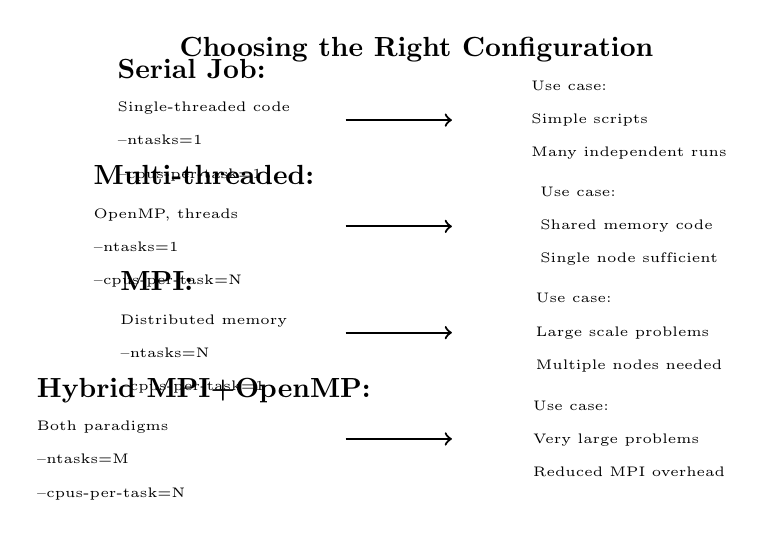
\begin{tikzpicture}[scale=0.9]
        % Header
        \node at (6, 6) {\textbf{Choosing the Right Configuration}};
        
        % Serial
        \node[align=left] at (3, 5) {
            \textbf{Serial Job:}\\
            \tiny Single-threaded code\\
            \tiny --ntasks=1\\
            \tiny --cpus-per-task=1
        };
        \draw[->, thick] (5, 5) -- (6.5, 5);
        \node[align=left] at (9, 5) {
            \tiny Use case:\\
            \tiny Simple scripts\\
            \tiny Many independent runs
        };
        
        % Multi-threaded
        \node[align=left] at (3, 3.5) {
            \textbf{Multi-threaded:}\\
            \tiny OpenMP, threads\\
            \tiny --ntasks=1\\
            \tiny --cpus-per-task=N
        };
        \draw[->, thick] (5, 3.5) -- (6.5, 3.5);
        \node[align=left] at (9, 3.5) {
            \tiny Use case:\\
            \tiny Shared memory code\\
            \tiny Single node sufficient
        };
        
        % MPI
        \node[align=left] at (3, 2) {
            \textbf{MPI:}\\
            \tiny Distributed memory\\
            \tiny --ntasks=N\\
            \tiny --cpus-per-task=1
        };
        \draw[->, thick] (5, 2) -- (6.5, 2);
        \node[align=left] at (9, 2) {
            \tiny Use case:\\
            \tiny Large scale problems\\
            \tiny Multiple nodes needed
        };
        
        % Hybrid
        \node[align=left] at (3, 0.5) {
            \textbf{Hybrid MPI+OpenMP:}\\
            \tiny Both paradigms\\
            \tiny --ntasks=M\\
            \tiny --cpus-per-task=N
        };
        \draw[->, thick] (5, 0.5) -- (6.5, 0.5);
        \node[align=left] at (9, 0.5) {
            \tiny Use case:\\
            \tiny Very large problems\\
            \tiny Reduced MPI overhead
        };
    \end{tikzpicture}
\end{frame}

\begin{frame}[fragile]{Job Arrays: Running Many Similar Jobs}
    \textbf{Scenario:} Need to run same program with different parameters
    \vskip1em
    \begin{columns}[T]
        \begin{column}{0.5\textwidth}
            \textbf{Without Job Arrays:}
            \begin{itemize}
                \item Submit 100 separate jobs
                \item Manage 100 job IDs
                \item Tedious and error-prone
            \end{itemize}
            \vskip1em
            \textbf{With Job Arrays:}
            \begin{itemize}
                \item Single submission
                \item One job ID with array indices
                \item Easier management
                \item Automatic resource scheduling
            \end{itemize}
        \end{column}
        \begin{column}{0.5\textwidth}
            \begin{lstlisting}[language=bash, basicstyle=\tiny\ttfamily]
#!/bin/bash
#SBATCH --job-name=array_job
#SBATCH --output=job_%A_%a.log
#SBATCH --array=1-100
#SBATCH --ntasks=1
#SBATCH --cpus-per-task=1
#SBATCH --mem=2G
#SBATCH --time=01:00:00

# SLURM_ARRAY_TASK_ID contains 
# the current array index (1-100)
PARAM=$SLURM_ARRAY_TASK_ID

echo "Processing parameter: $PARAM"
python process.py --id $PARAM
            \end{lstlisting}
            \vskip0.5em
            \textbf{Special variables:}
            \begin{itemize}
                \item \texttt{\%A}: Job array master ID
                \item \texttt{\%a}: Array task ID
                \item \texttt{\$SLURM\_ARRAY\_TASK\_ID}
            \end{itemize}
        \end{column}
    \end{columns}
\end{frame}

\begin{frame}[fragile]{Interactive Jobs with srun and salloc}
    \begin{columns}[T]
        \begin{column}{0.5\textwidth}
            \textbf{srun - Run single command:}
            \begin{lstlisting}[language=bash, basicstyle=\tiny\ttfamily]
# Interactive single command
srun --ntasks=1 \
     --cpus-per-task=4 \
     --mem=8G \
     --time=01:00:00 \
     python my_script.py
            \end{lstlisting}
            \begin{itemize}
                \item Blocks until complete
                \item Output to terminal
                \item Good for testing
            \end{itemize}
        \end{column}
        \begin{column}{0.5\textwidth}
            \textbf{salloc - Interactive shell:}
            \begin{lstlisting}[language=bash, basicstyle=\tiny\ttfamily]
# Allocate resources
salloc --nodes=1 \
       --ntasks=4 \
       --mem=16G \
       --time=02:00:00

# Now on compute node
hostname
module load python
python
# ... work interactively ...
exit  # Release resources
            \end{lstlisting}
            \begin{itemize}
                \item Interactive shell session
                \item Multiple commands
                \item Development and debugging
            \end{itemize}
        \end{column}
    \end{columns}
    \vskip1em
    \textbf{Note:} Interactive jobs consume resources even when idle. Use for active work only!
\end{frame}

%%%%%%%%%%%%%%%%%%%%%%%%%%%%%%%%%%%%%%%%%%%%%%%%%%%%%%%%%%%%%%%%%%%%%%%%%%
\section{Translating Concepts into Projects}
%%%%%%%%%%%%%%%%%%%%%%%%%%%%%%%%%%%%%%%%%%%%%%%%%%%%%%%%%%%%%%%%%%%%%%%%%%

\begin{frame}{Programming Languages and Parallel Computing}
    \begin{tabular}{p{2.5cm}p{3cm}p{5cm}}
        \toprule
        \textbf{Language} & \textbf{Paradigm} & \textbf{Common Tools} \\
        \midrule
        Python & Multi-threading & \texttt{threading}, \texttt{multiprocessing}, \texttt{joblib} \\
               & Message passing & \texttt{mpi4py} \\
               & Vectorization & \texttt{numpy}, \texttt{numba} \\
        \midrule
        Julia & Multi-threading & \texttt{Threads.@threads}, \texttt{@spawn} \\
              & Message passing & \texttt{MPI.jl} \\
              & Distributed & \texttt{Distributed.jl}, \texttt{@distributed} \\
        \midrule
        R & Multi-threading & \texttt{parallel}, \texttt{foreach} \\
          & Message passing & \texttt{Rmpi}, \texttt{pbdMPI} \\
          & Vectorization & Built-in vectorized operations \\
        \midrule
        C/C++ & Multi-threading & OpenMP, pthreads, TBB \\
              & Message passing & MPI \\
              & Vectorization & Compiler auto-vectorization \\
        \bottomrule
    \end{tabular}
\end{frame}

\begin{frame}[fragile]{Python: Multi-threading vs Multiprocessing}
    \begin{columns}[T]
        \begin{column}{0.5\textwidth}
            \textbf{Threading (GIL limitation):}
            \begin{lstlisting}[language=Python, basicstyle=\tiny\ttfamily]
from concurrent.futures import ThreadPoolExecutor
import numpy as np

def compute(x):
    # Good for I/O-bound tasks
    return np.sqrt(x)

with ThreadPoolExecutor(max_workers=4) as executor:
    results = executor.map(compute, range(100))
            \end{lstlisting}
            \vskip0.5em
            \textbf{Multiprocessing (True parallelism):}
            \begin{lstlisting}[language=Python, basicstyle=\tiny\ttfamily]
from multiprocessing import Pool

def compute(x):
    # Good for CPU-bound tasks
    return x ** 2

with Pool(processes=4) as pool:
    results = pool.map(compute, range(100))
            \end{lstlisting}
        \end{column}
        \begin{column}{0.5\textwidth}
            \textbf{Key Differences:}
            \begin{itemize}
                \item \textbf{Threading:} Shared memory, limited by GIL
                \item \textbf{Multiprocessing:} Separate processes, true parallelism
            \end{itemize}
            \vskip1em
            \textbf{SLURM Configuration:}
            \begin{lstlisting}[language=bash, basicstyle=\tiny\ttfamily]
# For multiprocessing
#SBATCH --ntasks=1
#SBATCH --cpus-per-task=4

# Set in Python
from multiprocessing import cpu_count
import os
n_cores = int(os.getenv(
    'SLURM_CPUS_PER_TASK', 
    cpu_count()))
            \end{lstlisting}
        \end{column}
    \end{columns}
\end{frame}

\begin{frame}[fragile]{Python: MPI with mpi4py}
    \textbf{Distributed memory parallelism in Python}
    \vskip1em
    \begin{columns}[T]
        \begin{column}{0.5\textwidth}
            \textbf{Example: Parallel computation}
            \begin{lstlisting}[language=Python, basicstyle=\tiny\ttfamily]
from mpi4py import MPI
import numpy as np

comm = MPI.COMM_WORLD
rank = comm.Get_rank()
size = comm.Get_size()

# Each process computes part
n_local = 1000
data = np.random.rand(n_local)
local_sum = np.sum(data)

# Reduce to get total sum
total_sum = comm.reduce(local_sum, 
                        op=MPI.SUM, 
                        root=0)

if rank == 0:
    print(f"Total: {total_sum}")
            \end{lstlisting}
        \end{column}
        \begin{column}{0.5\textwidth}
            \textbf{SLURM Job Script:}
            \begin{lstlisting}[language=bash, basicstyle=\tiny\ttfamily]
#!/bin/bash
#SBATCH --ntasks=16
#SBATCH --cpus-per-task=1
#SBATCH --mem-per-cpu=2G
#SBATCH --time=01:00:00

module load openmpi python/3.9

mpirun python my_mpi_script.py
            \end{lstlisting}
            \vskip0.5em
            \textbf{Key Points:}
            \begin{itemize}
                \item Use \texttt{mpirun} to launch
                \item Each process has unique rank
                \item Communication via MPI functions
                \item Scales across multiple nodes
            \end{itemize}
        \end{column}
    \end{columns}
\end{frame}

\begin{frame}[fragile]{Julia: Native Parallel Computing}
    \begin{columns}[T]
        \begin{column}{0.5\textwidth}
            \textbf{Multi-threading:}
            \begin{lstlisting}[language=Python, basicstyle=\tiny\ttfamily]
using Base.Threads

# Set threads with environment variable
# export JULIA_NUM_THREADS=4

function parallel_sum(arr)
    result = zeros(nthreads())
    @threads for i in eachindex(arr)
        tid = threadid()
        result[tid] += arr[i]
    end
    return sum(result)
end
            \end{lstlisting}
            \vskip0.5em
            \textbf{Distributed Computing:}
            \begin{lstlisting}[language=Python, basicstyle=\tiny\ttfamily]
using Distributed

addprocs(4)  # Add 4 workers

@everywhere function compute(x)
    return x^2
end

results = @distributed (+) for i = 1:100
    compute(i)
end
            \end{lstlisting}
        \end{column}
        \begin{column}{0.5\textwidth}
            \textbf{SLURM Configuration:}
            \begin{lstlisting}[language=bash, basicstyle=\tiny\ttfamily]
#!/bin/bash
#SBATCH --ntasks=1
#SBATCH --cpus-per-task=8
#SBATCH --mem=16G
#SBATCH --time=02:00:00

module load julia/1.8

# For threading
export JULIA_NUM_THREADS=$SLURM_CPUS_PER_TASK

julia my_script.jl
            \end{lstlisting}
            \vskip0.5em
            \textbf{MPI in Julia:}
            \begin{lstlisting}[language=Python, basicstyle=\tiny\ttfamily]
using MPI

MPI.Init()
comm = MPI.COMM_WORLD
rank = MPI.Comm_rank(comm)
size = MPI.Comm_size(comm)

# Parallel computation
            \end{lstlisting}
        \end{column}
    \end{columns}
\end{frame}

\begin{frame}[fragile]{R: Parallel Package}
    \begin{columns}[T]
        \begin{column}{0.5\textwidth}
            \textbf{Using foreach:}
            \begin{lstlisting}[language=Python, basicstyle=\tiny\ttfamily]
library(foreach)
library(doParallel)

# Register parallel backend
cl <- makeCluster(4)
registerDoParallel(cl)

# Parallel loop
results <- foreach(i=1:100, .combine=c) %dopar% {
    # Computation
    i^2
}

stopCluster(cl)
            \end{lstlisting}
            \vskip0.5em
            \textbf{Using mclapply:}
            \begin{lstlisting}[language=Python, basicstyle=\tiny\ttfamily]
library(parallel)

# Detect cores
ncores <- detectCores()

# Parallel apply
results <- mclapply(1:100, 
                    function(x) x^2,
                    mc.cores = ncores)
            \end{lstlisting}
        \end{column}
        \begin{column}{0.5\textwidth}
            \textbf{SLURM Job Script:}
            \begin{lstlisting}[language=bash, basicstyle=\tiny\ttfamily]
#!/bin/bash
#SBATCH --ntasks=1
#SBATCH --cpus-per-task=8
#SBATCH --mem=16G
#SBATCH --time=01:00:00

module load r/4.2

# Set cores from SLURM
export R_NCORES=$SLURM_CPUS_PER_TASK

Rscript my_script.R
            \end{lstlisting}
            \vskip0.5em
            \textbf{In R script:}
            \begin{lstlisting}[language=Python, basicstyle=\tiny\ttfamily]
# Get cores from environment
ncores <- as.integer(Sys.getenv("R_NCORES", "1"))

cl <- makeCluster(ncores)
# ... rest of code
            \end{lstlisting}
        \end{column}
    \end{columns}
\end{frame}

\begin{frame}{Debugging Parallel Programs}
    \begin{columns}[T]
        \begin{column}{0.5\textwidth}
            \textbf{Common Issues:}
            \begin{itemize}
                \item Race conditions
                \item Deadlocks
                \item Memory errors
                \item Load imbalance
                \item Communication bottlenecks
            \end{itemize}
            \vskip1em
            \textbf{Debugging Strategies:}
            \begin{itemize}
                \item Start with serial version
                \item Test with small problem size
                \item Use print statements
                \item Check with debuggers (GDB, DDT)
                \item Profile code performance
            \end{itemize}
        \end{column}
        \begin{column}{0.5\textwidth}
            \textbf{Best Practices:}
            \begin{enumerate}
                \item \textbf{Validate serial code first}
                \item \textbf{Start with small scale}
                \begin{itemize}
                    \item 2-4 processes/threads
                    \item Small data sets
                \end{itemize}
                \item \textbf{Compare results}
                \begin{itemize}
                    \item Serial vs parallel
                    \item Different core counts
                \end{itemize}
                \item \textbf{Use debugging tools}
                \begin{itemize}
                    \item Valgrind for memory
                    \item GDB for segfaults
                    \item profilers for performance
                \end{itemize}
                \item \textbf{Monitor resource usage}
                \begin{itemize}
                    \item Check CPU utilization
                    \item Memory consumption
                    \item Network traffic (MPI)
                \end{itemize}
            \end{enumerate}
        \end{column}
    \end{columns}
\end{frame}

\begin{frame}{Performance Optimization Tips}
    \begin{enumerate}
        \item \textbf{Profile Before Optimizing}
        \begin{itemize}
            \item Identify bottlenecks
            \item Focus on hot spots
            \item Measure, don't guess
        \end{itemize}
        
        \item \textbf{Optimize Serial Code First}
        \begin{itemize}
            \item Algorithm improvements
            \item Data structures
            \item Memory access patterns
        \end{itemize}
        
        \item \textbf{Minimize Communication}
        \begin{itemize}
            \item Reduce MPI calls
            \item Batch communications
            \item Overlap compute and communication
        \end{itemize}
        
        \item \textbf{Balance Load}
        \begin{itemize}
            \item Equal work distribution
            \item Dynamic load balancing
            \item Avoid idle processes
        \end{itemize}
        
        \item \textbf{Use Appropriate Tools}
        \begin{itemize}
            \item Vectorized operations
            \item Efficient libraries (BLAS, LAPACK)
            \item Compiler optimizations
        \end{itemize}
    \end{enumerate}
\end{frame}

\begin{frame}[fragile]{Scaling Studies}
    \begin{columns}[T]
        \begin{column}{0.5\textwidth}
            \textbf{Strong Scaling:}
            \begin{itemize}
                \item Fixed problem size
                \item Increase number of processors
                \item Measure time to solution
                \item Goal: Linear speedup
            \end{itemize}
            \vskip0.5em
            \textbf{Weak Scaling:}
            \begin{itemize}
                \item Fixed problem size per processor
                \item Increase processors and problem size together
                \item Measure time per processor
                \item Goal: Constant time
            \end{itemize}
        \end{column}
        \begin{column}{0.5\textwidth}
            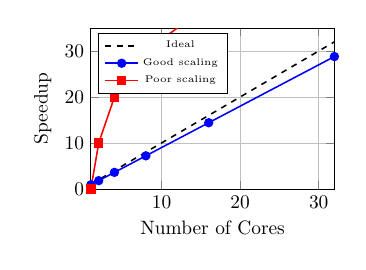
\begin{tikzpicture}[scale=0.7]
                \begin{axis}[
                    width=6cm,
                    height=4.5cm,
                    xlabel={Number of Cores},
                    ylabel={Speedup},
                    legend pos=north west,
                    grid=major,
                    xmin=1, xmax=32,
                    ymin=0, ymax=35,
                    legend style={font=\tiny}
                ]
                \addplot[black, dashed, thick, domain=1:32] {x};
                \addlegendentry{Ideal}
                
                \addplot[blue, thick, mark=*, samples at={1,2,4,8,16,32}] {x*0.9};
                \addlegendentry{Good scaling}
                
                \addplot[red, thick, mark=square*, samples at={1,2,4,8,16,32}] {10*log2(x)/log2(2)};
                \addlegendentry{Poor scaling}
                \end{axis}
            \end{tikzpicture}
            \vskip0.5em
            \textbf{Key Metrics:}
            \begin{itemize}
                \item Parallel efficiency = Speedup / N\_cores
                \item Aim for $>$80\% efficiency
            \end{itemize}
        \end{column}
    \end{columns}
\end{frame}

%%%%%%%%%%%%%%%%%%%%%%%%%%%%%%%%%%%%%%%%%%%%%%%%%%%%%%%%%%%%%%%%%%%%%%%%%%
\section{Q\&A and Interaction}
%%%%%%%%%%%%%%%%%%%%%%%%%%%%%%%%%%%%%%%%%%%%%%%%%%%%%%%%%%%%%%%%%%%%%%%%%%

\begin{frame}{Exercise 1: Writing Your First SLURM Script}
    \textbf{Task:} Create a simple SLURM job script
    \vskip1em
    \begin{enumerate}
        \item Create a script that:
        \begin{itemize}
            \item Prints the hostname
            \item Prints available environment variables
            \item Runs a simple calculation
        \end{itemize}
        \item Allocate: 1 node, 4 cores, 8GB RAM, 30 minutes
        \item Submit with \texttt{sbatch}
        \item Check status with \texttt{squeue}
        \item View output logs
    \end{enumerate}
    \vskip1em
    \textbf{Bonus:} Modify to use different core counts and compare timing
\end{frame}

\begin{frame}{Exercise 2: Parallel Python Script}
    \textbf{Task:} Write a parallel Python program
    \vskip1em
    \begin{enumerate}
        \item Create a script that:
        \begin{itemize}
            \item Computes sum of squares: $\sum_{i=1}^{N} i^2$
            \item Uses multiprocessing with 4 workers
            \item Compares with serial version
        \end{itemize}
        \item Measure execution time
        \item Create SLURM script to run it
        \item Experiment with different worker counts
    \end{enumerate}
    \vskip1em
    \textbf{Questions to explore:}
    \begin{itemize}
        \item How does speedup change with core count?
        \item What's the overhead of parallelization?
    \end{itemize}
\end{frame}

\begin{frame}{Exercise 3: Job Arrays}
    \textbf{Task:} Use job arrays for parameter sweep
    \vskip1em
    \begin{enumerate}
        \item Create a script that takes a parameter as input
        \item Run the same script with parameters 1-20
        \item Use SLURM job arrays
        \item Collect and analyze results
    \end{enumerate}
    \vskip1em
    \textbf{Example scenario:}
    \begin{itemize}
        \item Simulate with different random seeds
        \item Process different input files
        \item Test different hyperparameters
    \end{itemize}
    \vskip1em
    \textbf{Questions:}
    \begin{itemize}
        \item How to aggregate results from array jobs?
        \item What if some jobs fail?
    \end{itemize}
\end{frame}

\begin{frame}{Common Pitfalls and Solutions}
    \begin{tabular}{p{5cm}p{6cm}}
        \toprule
        \textbf{Pitfall} & \textbf{Solution} \\
        \midrule
        Job stuck in queue & Check node availability with \texttt{sinfo}; reduce resource requests \\
        Out of memory & Monitor with \texttt{sacct}; increase \texttt{--mem} \\
        Timeout & Increase \texttt{--time} or optimize code \\
        Wrong module & Use \texttt{module avail} and \texttt{module load} \\
        Poor parallel performance & Profile code; check CPU utilization \\
        Can't find output files & Check working directory; use absolute paths \\
        \bottomrule
    \end{tabular}
    \vskip1em
    \textbf{Debugging Tips:}
    \begin{itemize}
        \item Always check error logs first
        \item Test interactively with \texttt{salloc} or \texttt{srun}
        \item Start small, then scale up
    \end{itemize}
\end{frame}

\begin{frame}{Resource Estimation Guidelines}
    \textbf{How to estimate resources needed:}
    \vskip1em
    \begin{enumerate}
        \item \textbf{Memory:}
        \begin{itemize}
            \item Run small test with \texttt{/usr/bin/time -v}
            \item Check "Maximum resident set size"
            \item Add 20-30\% buffer
            \item Formula: $\text{mem} = \text{data\_size} \times \text{copies} \times 1.3$
        \end{itemize}
        
        \item \textbf{Time:}
        \begin{itemize}
            \item Time small problem
            \item Extrapolate to full size
            \item Add buffer for overhead
            \item Consider: $T_{\text{parallel}} \approx \frac{T_{\text{serial}}}{N_{\text{cores}} \times \text{efficiency}}$
        \end{itemize}
        
        \item \textbf{Cores:}
        \begin{itemize}
            \item Start with small counts (4-8)
            \item Measure speedup
            \item Check parallel efficiency
            \item Don't over-allocate
        \end{itemize}
    \end{enumerate}
\end{frame}

\begin{frame}{Best Practices Summary}
    \begin{columns}[T]
        \begin{column}{0.5\textwidth}
            \textbf{Job Submission:}
            \begin{itemize}
                \item Use descriptive job names
                \item Always specify time limits
                \item Use \texttt{\%j} in output files
                \item Test on small scale first
                \item Check queue before submitting many jobs
            \end{itemize}
            \vskip1em
            \textbf{Resource Usage:}
            \begin{itemize}
                \item Request what you need
                \item Don't monopolize resources
                \item Use job arrays for many similar jobs
                \item Clean up old files
            \end{itemize}
        \end{column}
        \begin{column}{0.5\textwidth}
            \textbf{Code Development:}
            \begin{itemize}
                \item Version control (git)
                \item Validate serial code first
                \item Test parallel code at small scale
                \item Profile before optimizing
                \item Document your workflow
            \end{itemize}
            \vskip1em
            \textbf{Data Management:}
            \begin{itemize}
                \item Use scratch space for temporary files
                \item Back up important results
                \item Compress large files
                \item Clean up after jobs
            \end{itemize}
        \end{column}
    \end{columns}
\end{frame}

\begin{frame}{Additional Resources}
    \textbf{Documentation:}
    \begin{itemize}
        \item SLURM Official Documentation: \texttt{https://slurm.schedmd.com/}
        \item Your cluster's wiki/documentation
        \item \texttt{man sbatch}, \texttt{man srun}, etc.
    \end{itemize}
    \vskip1em
    \textbf{Learning Resources:}
    \begin{itemize}
        \item HPC Carpentry: \texttt{https://www.hpc-carpentry.org/}
        \item XSEDE Training: \texttt{https://www.xsede.org/for-users/training}
        \item OpenMP Tutorial: \texttt{https://www.openmp.org/resources/tutorials-articles/}
        \item MPI Tutorial: \texttt{https://mpitutorial.com/}
    \end{itemize}
    \vskip1em
    \textbf{Tools:}
    \begin{itemize}
        \item Performance profilers: \texttt{gprof}, \texttt{perf}, \texttt{Intel VTune}
        \item Debuggers: \texttt{gdb}, \texttt{valgrind}, \texttt{DDT}
        \item Job monitoring: \texttt{squeue}, \texttt{sacct}, \texttt{scontrol}
    \end{itemize}
\end{frame}

\begin{frame}{Questions?}
    \begin{center}
        \Huge Thank You!
        \vskip2em
        \Large Questions and Discussion
        \vskip2em
        \normalsize
        \textbf{Contact Information:}\\
        {[}Your contact information here{]}
        \vskip1em
        \textbf{Cluster Support:}\\
        {[}Your HPC support contact here{]}
    \end{center}
\end{frame}

\end{document}
